\section{CMS overview}
\label{sec:CMS_overview}

In this section there will be an overview about Content Management Systems.

A Content Management System is an application, that provides capabilities for multiple users with different permission levels to manage content, data or information of a website project, or internet application \cite{cms_def}.

Managing content refers to creating, editing, archiving, publishing, collaborating on, reporting, distributing website content, data and information.
So, a CMS is an application that allows creating and publishing content from a central interface. CMSs are often used to run websites containing blogs, news, and shopping. Many corporate and marketing websites use CMSs. CMSs typically aim to avoid the need for hand coding, but may help it for specific elements or entire pages \cite{cms_over}. 

A Web CMS may catalog and index content, select or assemble content at runtime, or deliver content to specific visitors in a requested way, such as other languages. Web Content Management System's usually allow client control over HyperText Markup Language - based content, files, documents, and Web hosting plans based on the system depth and the niche it serves.


CMSs world involves three main actors: the developer, the admin and the user. Each figure plays a fundamental role in the life of a CMS managed website. The developer is the one who physically create the website, manage the functionality, design the graphics and make the set up to the administrator.
The administrator is non-technic a figure (not a programmer) who manage the website content: he can create, edit, publish and administer the material to show.
He manages the contents of the site through an administration panel that the developer created specifically. The administrator works into a reserved area, only accessible via a login panel.
Finally, the user is the one who benefits of the contents that the admin made avalaible. User can not access the administration panel and, therefore, can not create, edit or delete content (sometimes users can comment on existing content).

\begin {figure}[h]
\graphicspath{{images/chapter_cms/}}
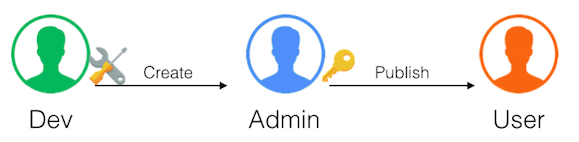
\includegraphics[width=\textwidth]{cms_schema}
\caption{CMS's actors schema}
\end {figure}


